\documentclass{tufte-handout}

%\geometry{showframe}% for debugging purposes -- displays the margins

\usepackage[spanish, es-tabla]{babel}
\usepackage{amsmath}
\usepackage{qf2}
\usepackage{physics}

% Set up the images/graphics package
\usepackage{graphicx}
\setkeys{Gin}{width=\linewidth,totalheight=\textheight,keepaspectratio}
\graphicspath{{figs/}{figs/retratos/}{graphics/}}

\title[Química Física II: Tema 5 - Átomos hidrogenoides]{
Tema 5: Átomos Hidrogenoides}
%\author{David De Sancho}
\date{}  % if the \date{} command is left out, the current date will be used

% The following package makes prettier tables.  We're all about the bling!
\usepackage{booktabs}

% The units package provides nice, non-stacked fractions and better spacing
% for units.
\usepackage{units}

% The fancyvrb package lets us customize the formatting of verbatim
% environments.  We use a slightly smaller font.
\usepackage{fancyvrb}
\fvset{fontsize=\normalsize}

% Small sections of multiple columns
\usepackage{multicol}

% Retratos históricos en el margen. Todas las imágenes son de dominio
% público y proceden de Wikimedia Commons; la procedencia completa está en
% figs/retratos/CREDITOS.md.
%
% Es un marginfigure SIN \caption: así no consume números de figura y no
% desplaza los \ref existentes. El % tras el corchete no es opcional (sin él
% la imagen se sale del margen). El razonamiento completo está comentado en
% el preámbulo de tema01.tex.
\makeatletter
\setlength{\@fptop}{0pt}
\makeatother

\newcommand{\retrato}[2]{%
  \begin{marginfigure}[\baselineskip]%
    \includegraphics[width=\linewidth]{#1}\par
    \vspace{0.4ex}{\footnotesize #2}\par
    \vspace*{\baselineskip}
  \end{marginfigure}}

\begin{document}

\maketitle% this prints the handout title, author, and date

\begin{abstract}
\noindent Tras describir una serie de sistemas modelo, aplicamos ahora
sus soluciones al estudio de sistemas relevantes para la Química. En primer lugar, estudiaremos 
átomos hidrogenoides, es decir, átomos con tan sólo un
electrón (H, He$^+$, Li$^{2+}$, O$^{7+}$\ldots). La importancia
de estos sistemas radica, en parte, en que su ecuación de
Schrödinger tiene solución exacta.
\end{abstract}


\section{Unidades atómicas}
En este tema, a menudo nos resultará de utilidad expresar las 
magnitudes en unidades atómicas, es decir, normalizando la carga, 
la masa, la longitud, el momento angular o la energía, por los 
valores que mostramos en la Tabla~\ref{tb:au}.

\begin{table}[h!]
    \centering
    \small{}
    \setlength{\tabcolsep}{3pt}
    \begin{tabular}{|l|l|c|l|}
    \hline
         Propiedad & Unidad & Equivalencia SI& Nombre  \\
    \hline
    \hline
         Carga elemental & $e$ & $1.602\times10^{-19}$ C & \\ 
         Masa & $m_e$ & $9.109\times10^{-31}$ kg & \\ 
         Momento angular & $\hbar$ & $1.055\times10^{-34}$ J$\cdot$s & \\ 
         Constante eléctrica & $4\pi \varepsilon_0$ & $1.113\times10^{-10}$ C$^2\cdot$J$^{-1}\cdot$m$^{-1}$ & \\
         Longitud & $a_0=4\pi \varepsilon_0\hbar^2/m_ee^2$ & $5.291\times10^{-11}$ m & bohr \\ 
         Energía & $E_h=e^2/4\pi \varepsilon_0a_0$  & $4.359\times10^{-18}$ J & hartree \\ 
    \hline
    \end{tabular}
    \caption{Conversión entre unidades atómicas y del SI.}
    \label{tb:au}
\end{table}

\section{Hamiltoniano para el átomo hidrogenoide}
En este caso podremos reducir el problema a la suma de dos problemas 
más sencillos de una sola partícula. Por un lado, el sistema se 
desplaza como si toda la masa estuviera concentrada en un solo punto,
el centro de masas. Por otra parte, podemos describir el movimiento 
relativo de rotación y vibración de una partícula ficticia sometida 
a un potencial central. Esta simplificación no se puede aplicar en 
general a problemas de tres o más cuerpos.

Para átomos hidrogenoides el hamiltoniano es
\begin{equation}
    \hat{H}=\hat{K}_N(\mathbf{R}_N) + \hat{K}_e(\mathbf{r}_e) + \hat{V}_{eN}(r_{eN})
\end{equation}
donde el primer y segundo término en el lado derecho de la ecuación 
corresponden a la energía cinética del núcleo y del electrón, 
respectivamente, y el último término es el potencial electrostático 
entre núcleo y electrón. 

Si separamos el movimiento del centro de masas, de masa total
$M$, del movimiento relativo, la parte correspondiente al centro
de masas la podremos resolver usando un modelo como el de la
partícula libre. Por tanto, nos podemos centrar en los términos 
correspondientes al movimiento relativo del electrón en torno
al núcleo y la atracción entre núcleo y electrón. Desarrollando 
los diferentes términos y usando las soluciones del Tema 4,
obtenemos
\begin{equation}
    \hat{H}=-\frac{\hbar^2}{2\mu}\nabla_r^2+ \frac{\hat{l}^2}{2\mu r^2} - \frac{Ze^2}{4\pi \varepsilon_0r}
\end{equation}
donde el primer término del miembro derecho
contiene la contribución radial del hamiltoniano, el segundo 
término corresponde a la parte angular y el último término
representa la interacción electrostática núcleo-electrón.
El operador $\hat{H}$ conmuta con $\hat{l}_z$ y $\hat{l}^2$. Estos
operadores tienen funciones propias comunes y los estados estacionarios
se pueden caracterizar por $E$, $l^2$ y $l_z$. 

\section{Soluciones de la ecuación de Schrödinger}
Dado que la energía potencial es centrosimétrica (independiente
de la componente angular), la ecuación de Schrödinger es separable
en componentes radial y angular. Así, las funciones de onda
hidrogenoides, denominadas \textbf{orbitales atómicos},\sidenote{El
término \textit{orbital} lo propuso Robert S. Mulliken en 1932 para
referirse a la función de onda de un solo electrón.} son de la forma
\begin{equation}
    \psi=R_{n,l}(r)Y_{l,m_l}(\theta,\phi)
\end{equation}


\subsection{Solución de la parte angular}
Empezamos por la parte angular, 
\begin{equation}
    \Lambda^2Y=-l(l+1)Y
\end{equation}
que ya resolvimos en el tema anterior. Las funciones angulares $Y$ 
son los armónicos esféricos, especificados por los números cuánticos
angular ($l$) y magnético ($m_l$). Estas funciones dependen sólo
de la dirección ($\theta,\phi$), no de la distancia $r$. 


\subsection{Solución radial}
La parte radial de la ecuación de Schrödinger es
\begin{equation}
    \bigg\{-\frac{\hbar^2}{2\mu r^2}\frac{\partial}{\partial r}\bigg(r^2\frac{\partial}{\partial r}\bigg) 
    +  \frac{l(l+1)\hbar^2}{2\mu r^2}
    - \frac{Ze^2}{4\pi \varepsilon_0r}  \bigg\}
    R(r)
    = ER(r)
\end{equation}
Aunque no vamos a desarrollar la solución de esta ecuación, la función
radial tiene la siguiente estructura
\begin{equation}
    R(r)=(\textrm{polinomio en }r)\times(\textrm{exponencial en }r)
\end{equation}
Estas funciones radiales se expresan con mayor facilidad 
en función de la magnitud adimensional $\rho$, que definimos como
\begin{equation}
    \rho = \frac{2Zr}{na_0}
\end{equation}
En concreto, la forma funcional, dependiente de los números
cuánticos principal ($n$) y angular ($l$), es la siguiente
\begin{equation}
  R_{n,l} = N_{n,l}\rho^l L^{2l+1}_{n+l}(\rho)\exp(-\rho/2)
\end{equation}
donde $n=1,2,3,\ldots$ y $l=0,\ldots,n-1$, y $L$ es un polinomio
asociado de Laguerre. A pesar de la complejidad de esta función,
los polinomios dependientes de $n$ y $l$ son relativamente
sencillos. 

Mostramos las 
funciones resultantes para los primeros números cuánticos en
la Tabla~\ref{tb:radial_hydrogenoid}. El factor exponencial
hace que $R$ tienda a cero lejos del núcleo; el factor $\rho^l$
la anula en el núcleo cuando $l>0$; y el polinomio de Laguerre la
hace oscilar entre valores positivos y negativos, con $n-l-1$
nodos radiales. A estos se suman los
$l$ nodos angulares de los armónicos esféricos, de modo que el
número total de nodos es $n-1$ (Figura~\ref{fig:radiales}). 

\begin{figure*}[!htb]
  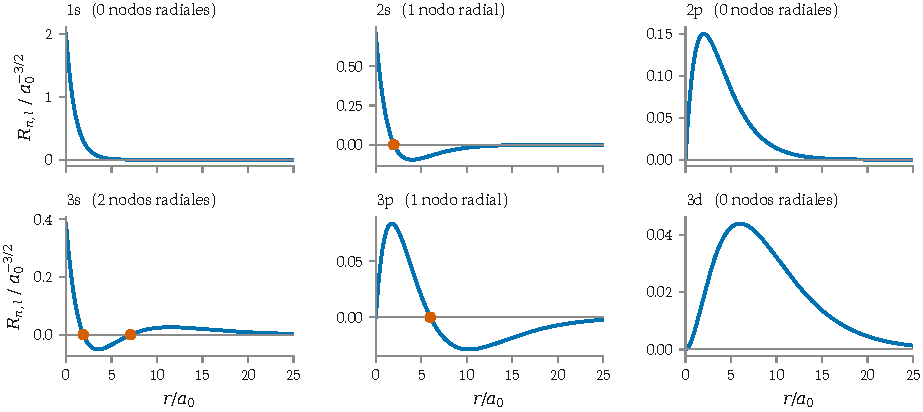
\includegraphics{hidrogeno_radial_Rnl_v1.pdf}
  \caption{Funciones radiales $R_{n,l}(r)$ del hidrógeno ($Z=1$) para
  $n\le 3$. Los puntos marcan los nodos radiales, cuyo número es $n-l-1$.}
  \label{fig:radiales}
\end{figure*}
\begin{table}[b!]
    \centering
    \begin{tabular}{|c|c|c|c|}
    \hline
         Orbital & $n$  & $l$ &$R_{n,l}$ \\
    \hline
    \hline
         1s & 1 & 0 & 
         $2\bigg(\frac{Z}{a}\bigg)^{3/2}\mathrm{e}^{-\rho/2}$ \\
         2s & 2 & 0 & 
         $\frac{1}{8^{1/2}}\bigg(\frac{Z}{a}\bigg)^{3/2}(2-\rho) \mathrm{e}^{-\rho/2}$\\
         2p & 2 & 1 & 
         $\frac{1}{24^{1/2}}\bigg(\frac{Z}{a}\bigg)^{3/2}\rho \mathrm{e}^{-\rho/2}$\\
         3s & 3 & 0 & 
         $\frac{1}{243^{1/2}}\bigg(\frac{Z}{a}\bigg)^{3/2}(6-6\rho+\rho^2)\mathrm{e}^{-\rho/2}$ \\
         3p & 3 & 1 &
         $\frac{1}{486^{1/2}}\bigg(\frac{Z}{a}\bigg)^{3/2}(4-\rho)\rho \mathrm{e}^{-\rho/2}$ \\
         3d & 3 & 2 & $\frac{1}{2430^{1/2}}\bigg(\frac{Z}{a}\bigg)^{3/2}\rho^2\mathrm{e}^{-\rho/2}$ \\
    \hline
    \end{tabular}
    \caption{Funciones de onda radiales de átomos hidrogenoides. En estas expresiones, 
    usamos $a=4 \pi \varepsilon_0\hbar^2/\mu e^2$.}
    \label{tb:radial_hydrogenoid}
\end{table}



Asimismo llegamos a expresiones compactas para la energía de 
los estados ligados de los átomos hidrogenoides
\begin{equation}
    E_n=-\frac{Z^2\mu e^4}{32\pi^2\varepsilon_0^2\hbar^2 n^2}
    \label{eq:Eh}
\end{equation}
que dependen exclusivamente del número cuántico $n$. 
En el caso del hidrógeno, podemos aproximar la masa reducida
a la masa del electrón $\mu\simeq m_e$. 

\section{Orbitales atómicos del hidrógeno}
A partir de la función de onda podemos derivar las 
propiedades de los orbitales del átomo de hidrógeno, 
caracterizados por los tres números cuánticos $n$, $l$ y
$m_l$. Cuando un electrón ocupa un orbital descrito por la
función de onda $\psi_{n,l,m_l}$, decimos que se
encuentra en el estado $|n,l,m_l\rangle$.

El número cuántico principal
es $n$, que puede tomar valores enteros $n=1,2,3,\ldots$
y determina la energía del electrón, descrita por la Ecuación~\ref{eq:Eh}.
Todas las energías de los estados ligados del átomo son negativas,
es decir, inferiores a la del electrón infinitamente separado
del núcleo que corresponde al cero en energía.

Los otros dos números cuánticos, $l$ y $m_l$, proceden de la solución
angular y especifican el momento angular del electrón en torno al 
núcleo. Un electrón con número cuántico $l$ tiene un momento angular
de magnitud $\{l(l+1)\}^{1/2}\hbar$, con $l=0,1,2,\ldots,n-1$. 
Sin embargo, las tres componentes del momento angular no pueden
conocerse simultáneamente, porque los operadores correspondientes no
conmutan entre sí. Sí podemos conocer a la vez la magnitud y una de las
componentes, que por convenio es la componente $z$, cuyo valor es
$l_z=m_l\hbar$, con $m_l=0,\pm 1,\ldots,\pm l$.

\subsection{Capas y subcapas}
Las funciones con un número cuántico principal común $n$
tienen la misma energía y su región de máxima densidad a distancias
muy similares. Esto da lugar a una estructura de capas. Los orbitales
con $n=1,2,3,4,\ldots$ forman las capas $K$, $L$, $M$ y $N$, respectivamente.
Los orbitales con el mismo número cuántico principal pero diferente 
número cuántico $l$ forman subcapas correspondientes a $l=0,1,2,3,4,\ldots$,
llamadas $s$, $p$, $d$, $f$, $g$\ldots\sidenote{El origen de las letras \textit{s},
\textit{p}, \textit{d} y \textit{f} ---para ``sharp'', ``principal'', ``diffuse'' y ``fundamental'', respectivamente---
está relacionado con las líneas espectrales del átomo de sodio.}
Para una capa con número cuántico 
$n$, hay un total de $n$ subcapas (de 0 hasta $n-1$). El número de 
orbitales atómicos en una capa correspondiente al número cuántico 
principal $n$ es $n^2$, con lo cual en un átomo hidrogenoide
la degeneración energética es de $n^2$ (Figura~\ref{fig:niveles}).

\begin{figure}[!htb]
  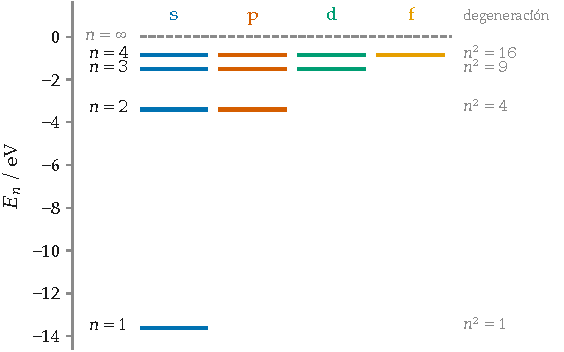
\includegraphics{hidrogeno_niveles-degeneracion_v1.pdf}
  \caption{Niveles de energía del hidrógeno, $E_n=-13.6/n^2$ eV, para
  $n\le 4$. La energía depende sólo de $n$: todas las subcapas de una capa
  están a la misma altura, y la degeneración de la capa es $n^2$, la suma
  de las $2l+1$ funciones de cada subcapa. La línea discontinua marca el
  límite de ionización.}
  \label{fig:niveles}
\end{figure}

\subsection{Geometría de los orbitales atómicos}
El orbital ocupado en el estado fundamental es el que tiene $n=1$
y $l=m_l=0$. El valor de $R$ lo podemos tomar de la Tabla~\ref{tb:radial_hydrogenoid} y la función de onda angular en 
este caso es una constante, $Y_{0,0}=1/\sqrt{4\pi}$.
Esto da lugar a la función de onda 
\begin{equation}
    \psi=\bigg(\frac{Z^3}{\pi a_0^3}\bigg)^{1/2}\mathrm{e}^{-Zr/a_0}
\end{equation}
con simetría esférica que decae exponencialmente desde un máximo
que se encuentra en el núcleo ($r=0$). Por tanto la \textbf{densidad 
electrónica} $|\psi_{n,l,m_l}|^2=R^2_{n,l}|Y_{l,m_l}|^2$ 
será máxima en el núcleo mismo y decaerá al alejarnos de él. 
En el caso de los orbitales p ($l=1$) la función angular no 
es constante y la probabilidad de encontrar el electrón a 
una distancia $r$ difiere en función de la orientación
(Figura~\ref{fig:densidad-2d}).

\begin{figure*}[!htb]
  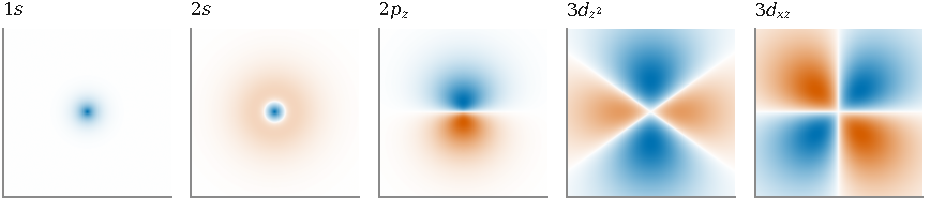
\includegraphics{hidrogeno_densidad-2d_v1.pdf}
  \caption{Cortes en el plano $xz$ de los orbitales 1s, 2s, 2p$_z$,
  3d$_{z^2}$ y 3d$_{xz}$ del hidrógeno, en un mismo recuadro de $32a_0$ de
  lado. La intensidad del color es proporcional a $|\psi|^{0.7}$, una
  escala realzada que hace visibles las regiones de baja densidad, y el
  color indica el signo de $\psi$: azul positivo, naranja negativo. Las
  líneas blancas son los nodos: una esfera (nodo radial) en el 2s; planos
  o conos (nodos angulares) en los orbitales p y d.}
  \label{fig:densidad-2d}
\end{figure*}

La función de onda nos dice, a partir del valor de $|\psi_{n,l,m_l}|^2$,
la probabilidad de encontrar el electrón en una región determinada.
Si queremos calcular la probabilidad de encontrar el electrón
en una región correspondiente a un casquete esférico ubicado 
a una distancia $r$ del núcleo y con grosor $dr$ y volumen 
$4\pi r^2dr$ entonces debemos calcular la \textbf{función de distribución 
radial}
\begin{equation}
    P(r)=r^2R(r)^2
\end{equation}
que es válida para cualquier orbital. En el caso de los orbitales s
($l=0$), $Y_{0,0}=1/\sqrt{4\pi}$ y la expresión se reduce a
\begin{equation}
    P(r)=4\pi r^2\psi^2(r)
\end{equation}
El producto $P(r)\,dr$ es la probabilidad de encontrar el electrón
en el casquete esférico comprendido entre $r$ y $r+dr$. Para un orbital 1s, el valor de la función de
distribución radial es 
\begin{equation}
    P(r)=\frac{4Z^3}{a_0^3}r^2\exp(-2Zr/a_0)
\end{equation}
A partir de esta expresión vemos que en el núcleo, donde
$r=0$ y por tanto $r^2=0$, $P(0)=0$. Lejos del núcleo, $r\to\infty$,
$P(r)$ también tiende a cero. Entre ambos extremos la función tiene un
máximo, cuya posición obtenemos igualando a cero su derivada. En particular, en el caso del orbital 1s el máximo se
encuentra en $r=a_0/Z$, es decir, en $r=a_0$ para el hidrógeno. Para el
orbital 2s, el radio más probable está en $5.2a_0/Z$. En la
Figura~\ref{fig:rdf} mostramos la función de distribución radial de los
orbitales de las tres primeras capas.

\begin{figure*}[!htb]
  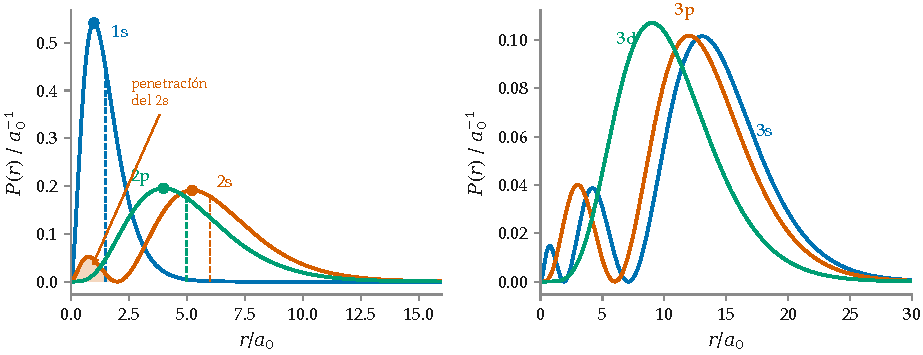
\includegraphics{hidrogeno_rdf_1s-3d_v1.pdf}
  \caption{Funciones de distribución radial $P(r)=r^2R_{n,l}^2$ del
  hidrógeno. Izquierda: orbitales 1s, 2s y 2p; los puntos marcan el radio
  más probable y las líneas discontinuas el radio medio $\langle r\rangle$
  (para el 1s, $a_0$ y $1.5a_0$). La zona sombreada es la penetración del
  2s: parte de su densidad se encuentra muy cerca del núcleo, donde el 2p
  apenas llega. Derecha: capa $n=3$; a igual $n$, cuanto menor es $l$, más
  penetra el orbital.}
  \label{fig:rdf}
\end{figure*} 

\FloatBarrier
\section{Efecto Zeeman}
En 1896, Pieter Zeeman descubrió que un campo magnético desdobla las
líneas espectrales de los átomos. Este \textbf{efecto Zeeman} surge de la interacción entre el campo magnético aplicado y los
momentos magnéticos debidos al momento angular orbital y de espín.

Para entender este efecto, es importante
que recordemos conceptos fundamentales de magnetismo. En general, el
momento magnético $\boldsymbol{\mu}$ generado por una carga eléctrica $q$
de masa $m$ que gira en una órbita se expresa como
\begin{equation}
    \boldsymbol{\mu}=\frac{q(\mathbf{r}\times\mathbf{v})}{2}
\end{equation}
donde $\mathbf{r}$ y $\mathbf{v}$ son los vectores posición y velocidad
correspondientes a la carga. El momento magnético se puede expresar en
términos del momento angular, $\mathbf{l}=\mathbf{r}\times\mathbf{p}$,
para obtener
\begin{equation}
    \boldsymbol{\mu}=\frac{q}{2m}\mathbf{l}
\end{equation}
donde tanto $\boldsymbol{\mu}$ como $\mathbf{l}$ son perpendiculares al plano 
de movimiento. Particularizando para el caso del electrón, obtenemos
\begin{equation}
    \boldsymbol{\mu}=-\frac{e}{2m_e}\mathbf{l}
\end{equation}

La energía potencial asociada a la interacción de un momento magnético
con un campo magnético $\mathbf{B}$ viene dada por 
\begin{equation}
    V=-\boldsymbol{\mu}\cdot\mathbf{B}
\end{equation}
Normalmente, tomamos el eje $z$ en la dirección del campo,
por lo que el potencial pasa a ser
\begin{equation}
    V=-\mu_zB_z=\frac{eB_z}{2m_e}l_z
\end{equation}
\retrato{retrato_zeeman_v1.jpg}{Pieter Zeeman (1865--1943) en 1902, año
en que compartió el premio Nobel de Física con Hendrik Lorentz.}%
Si remplazamos $l_z$ por el correspondiente operador $\hat{l}_z$,
podemos añadir este término de energía potencial para 
escribir el operador hamiltoniano en presencia de un campo
magnético
\begin{equation}
    \hat{H}=\hat{H}_0 + \frac{eB_z}{2m_e}\hat{l}_z
\end{equation}
donde $\hat{H}_0$ es el hamiltoniano en ausencia de un campo
magnético.

Los orbitales atómicos son funciones propias tanto del operador
$\hat{H}_0$ como del operador $\hat{l}_z$. Por consiguiente, 
lo son también del operador $\hat{H}$. Las energías asociadas
a los orbitales en presencia del campo magnético son
\begin{equation}
    E=E_n + \mu_Bm_lB_z \label{eq:ener_zeeman}
\end{equation}
donde hemos definido el magnetón de Bohr, 
$\mu_B=e\hbar/2m_e=9.274\times10^{-24}$ J T$^{-1}$.
En términos del magnetón de Bohr, la componente $z$ del momento
magnético orbital del electrón es simplemente $\mu_z=-\mu_Bm_l$.
En ausencia de un campo magnético la energía de un
átomo de hidrógeno es independiente del número cuántico $m_l$.
En presencia del campo, en cambio, depende de $m_l$ y es por tanto
diferente para las posibles orientaciones del vector momento angular
(Figura~\ref{fig:zeeman}).
\begin{marginfigure}
  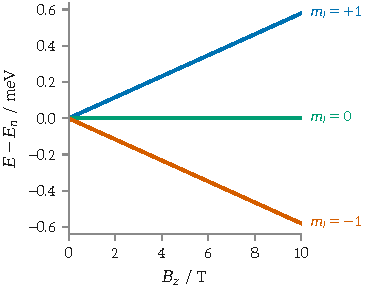
\includegraphics{zeeman_desdoblamiento_l1_v1.pdf}
  \caption{Desdoblamiento Zeeman de un nivel con $l=1$,
  $E-E_n=\mu_Bm_lB_z$. Incluso a 10 T la separación entre subniveles
  contiguos es de sólo 0.58 meV.}
  \label{fig:zeeman}
\end{marginfigure}

El efecto Zeeman rompe la degeneración energética
de los orbitales. Supongamos un estado con valores de los números 
cuánticos $n$ y $l$. A partir de la Ecuación~\ref{eq:Eh} todos los
orbitales tendrían la misma energía. Sin embargo, dado que este estado
tiene $2l+1$ valores de $m_l$, en presencia de un campo magnético estará 
dividido en $2l+1$ niveles, cuyos valores vendrán dados por la
Ecuación~\ref{eq:ener_zeeman}.

Un estado s de un átomo de hidrógeno no experimenta este desdoblamiento.
Pero el estado p se divide en tres subniveles, correspondientes
a las diferentes orientaciones de $l_z$. De acuerdo con esto, al aplicar 
un campo magnético a un átomo de hidrógeno en su estado fundamental (1s), 
su energía no debería cambiar. Sin embargo, experimentalmente se observa
que el nivel 1s se desdobla en dos subniveles, lo cual indica que el
electrón tiene un momento magnético adicional, que no procede de su
movimiento orbital. Del mismo modo, en muchos átomos las líneas
espectrales se desdoblan en presencia de un campo magnético en un número
de componentes distinto del que predice la Ecuación~\ref{eq:ener_zeeman}.
Este comportamiento se conoce como \textbf{efecto Zeeman anómalo}, y sólo
pudo explicarse tras la introducción del espín electrónico, que veremos
a continuación.

\section{Stern--Gerlach y el espín electrónico}
La influencia de los campos magnéticos sobre el átomo no concluye 
con el efecto Zeeman. En 1921, el físico estadounidense Arthur H. Compton
afirmaba que ``el electrón, girando sobre sí mismo como un pequeño
giroscopio, es probablemente la partícula magnética elemental''.
Un año más tarde, Otto Stern y Walther Gerlach realizaron un célebre
experimento: hicieron pasar un haz de átomos de plata
(4d$^{10}$5s$^1$, con un único electrón de valencia) a través de un
campo magnético no homogéneo y observaron que el haz se desdoblaba en dos bandas.
Por tanto, los átomos de plata debían tener un momento
magnético cuya orientación con respecto al eje $z$ estaba cuantizada. 
Estas dos bandas contradecían las $2l+1$ orientaciones posibles del
momento angular determinado por $l$. Además, la aparición de dos 
bandas sugería un valor de $l=1/2$, en lugar de los valores 
enteros de $l$ permitidos.

\retrato{retrato_stern_v1.jpg}{Otto Stern (1888--1969) hacia 1940.
Recibió el premio Nobel de Física de 1943.}%
En 1925, Wolfgang Pauli propuso que estas observaciones podrían
explicarse si el electrón existía en dos estados diferenciables. 
Pauli introdujo \textit{ad hoc} un misterioso 
cuarto número cuántico, $m_s$,
restringido a tener valores de $m_s=\pm 1/2$, aunque no le dio
interpretación alguna.
Los físicos holandeses Goudsmit y Uhlenbeck propusieron el mismo año 
la existencia de un momento angular intrínseco del electrón, que fue
denominado momento angular de \textbf{espín}. Su módulo es 
\begin{equation}
    |\mathbf{s}|=\sqrt{s(s+1)}\hbar
\end{equation}
y su componente en el eje $z$ es $s_z=m_s\hbar$, donde $m_s=-s,\ldots,s$.
En el caso del electrón, $s=1/2$, lo que da lugar a dos orientaciones
posibles: $m_s=+1/2$, o espín hacia arriba y $m_s=-1/2$ o
espín hacia abajo. Las funciones de onda de espín, $\alpha$ y $\beta$,
respectivamente, son ortonormales
\begin{align}
    \int\alpha^\star\alpha d\sigma=\int \beta^\star\beta d\sigma=1 \\
    \int\alpha^\star\beta d\sigma=\int \beta^\star\alpha d\sigma=0 
\end{align}
o en notación de Dirac
\begin{align}
    \bra{\alpha}\ket{\alpha}= \bra{\beta}\ket{\beta}=1\\
    \bra{\alpha}\ket{\beta}= \bra{\beta}\ket{\alpha}=0
\end{align}

Al incluir el espín obtenemos la función de onda completa del
electrón, el \textbf{espín-orbital}, producto de la parte espacial
(radial y angular) y de una función de espín
\begin{align}
\Psi_{n,l,m_l,m_s}(r,\theta,\phi,\sigma)=\psi_{n,l,m_l}(r,\theta,\phi)\alpha(\sigma) \\
\Psi_{n,l,m_l,m_s}(r,\theta,\phi,\sigma)=\psi_{n,l,m_l}(r,\theta,\phi)\beta(\sigma) 
\end{align}
o en notación de Dirac, $\ket{n,l,m_l,m_s}$.
\end{document}
